\documentclass[aspectratio=169,11pt]{beamer}
\usepackage[T1]{fontenc}
\usepackage{lmodern,amsmath,booktabs,graphicx,tikz}
\usetheme[progressbar=frametitle,numbering=fraction,sectionpage=none]{metropolis}
\definecolor{Ink}{HTML}{172D3A}
\definecolor{Muted}{HTML}{405864}
\definecolor{Teal}{HTML}{007465}
\definecolor{Rust}{HTML}{AD482B}
\definecolor{Wash}{HTML}{EDF5F3}
\definecolor{Rule}{HTML}{CFDEDE}

\newcommand{\ModelMetric}[3]{\csname metric:#1:#2:#3\endcsname}
\newcommand{\ModelMeanADEChange}[2]{\csname delta:#1:#2\endcsname}
\newcommand{\ModelRuntime}[2]{\csname runtime:#1:#2\endcsname}
\input{generated/model-metrics.tex}
\input{generated/submission-status.tex}

\setbeamersize{text margin left=0.85cm,text margin right=0.85cm}
\setbeamercolor{normal text}{fg=Ink,bg=white}
\setbeamercolor{palette primary}{fg=white,bg=Ink}
\setbeamercolor{alerted text}{fg=Rust}
\setbeamercolor{progress bar}{fg=Teal,bg=Rule}
\setbeamercolor{title separator}{fg=Teal}
\setbeamertemplate{navigation symbols}{}

\begin{document}
\begin{frame}[plain,noframenumbering]{}
\noindent
{\small\color{Teal}\bfseries COMP5331 GROUP 7 \hfill FALL 2026\par}
\vspace{0.9cm}
{\bfseries\fontsize{29}{33}\selectfont Pedestrian trajectory\\forecasting\par}
\vspace{0.15cm}
{\color{Teal}\rule{0.94\linewidth}{0.9pt}\par}
\vspace{0.22cm}
{\large Six independent implementations on ETH/UCY\par}
\vspace{0.65cm}
{\small\color{Muted}\SubmissionStatus\par}
\end{frame}

\begin{frame}{All models receive the same observed windows}
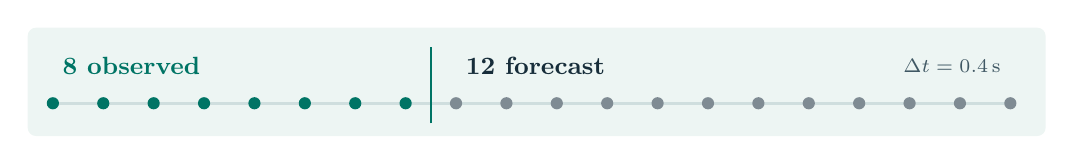
\begin{tikzpicture}[x=0.64cm,y=0.64cm]
\fill[Wash,rounded corners=3pt] (-.5,-.65) rectangle (19.7,1.50);
\draw[Rule,line width=1pt] (0,0) -- (19,0);
\foreach \x in {0,...,7}{\fill[Teal] (\x,0) circle (2.2pt);}
\foreach \x in {8,...,19}{\fill[Ink!55] (\x,0) circle (2.2pt);}
\draw[Teal,thick] (7.5,-.40) -- (7.5,1.12);
\node[Teal,anchor=west,font=\small\bfseries] at (0,.74) {8 observed};
\node[Ink,anchor=west,font=\small\bfseries] at (8,.74) {12 forecast};
\node[Muted,anchor=east,font=\scriptsize] at (19,.74) {$\Delta t=0.4$\,s};
\end{tikzpicture}

\medskip
\begin{columns}[T,onlytextwidth]
\column{.31\textwidth}
\textcolor{Teal}{\bfseries Generalization}\par\smallskip
Five held-out scenes and three seeds. Select checkpoints on validation.
\column{.31\textwidth}
\textcolor{Teal}{\bfseries Robustness}\par\smallskip
Compare target-only position noise and missing-suffix conditions.
\column{.31\textwidth}
\textcolor{Teal}{\bfseries Distribution}\par\smallskip
Separate typical error from best-of-\(K\). Report sample budget and Energy Score.
\end{columns}
\end{frame}

\input{generated/model-slides.tex}

\begin{frame}{Clean results are reported at explicit sample budgets}
\centering
\small
\renewcommand{\arraystretch}{1.08}
\begin{tabular}{lrrrrrr}
\toprule
Model & \(K\) & minADE & minFDE & meanADE & meanFDE & ES \\
\midrule
\input{generated/comparison-rows.tex}
\end{tabular}

\vspace{0.28cm}

{\footnotesize\color{Muted}Equal-weight holdout means in meters. Read minimum error at the stated \(K\).}
\end{frame}

\IfFileExists{editor/slides_synthesis.tex}{\begin{frame}{Position noise raised mean ADE more than two missing points}
\centering
\small
\begin{tabular}{lrrr}
\toprule
Model & \(K\) & 0.20\,m noise & Two missing \\
\midrule
Individual LSTM & 1 & \ModelMeanADEChange{individual_lstm}{noise_020} & \ModelMeanADEChange{individual_lstm}{missing_2} \\
Social-LSTM & 1 & \ModelMeanADEChange{social_lstm}{noise_020} & \ModelMeanADEChange{social_lstm}{missing_2} \\
Social-GAN & 20 & \ModelMeanADEChange{social_gan}{noise_020} & \ModelMeanADEChange{social_gan}{missing_2} \\
Social-STGCNN & 20 & \ModelMeanADEChange{social_stgcnn}{noise_020} & \ModelMeanADEChange{social_stgcnn}{missing_2} \\
Trajectron++ & 20 & \ModelMeanADEChange{trajectronpp}{noise_020} & \ModelMeanADEChange{trajectronpp}{missing_2} \\
DSPIGCN & 20 & \ModelMeanADEChange{dspigcn}{noise_020} & \ModelMeanADEChange{dspigcn}{missing_2} \\
\bottomrule
\end{tabular}

\medskip
{\footnotesize\color{Muted}Paired mean ADE change from clean input, in meters.}
\end{frame}
}{}
\end{document}
